% Template for IGARSS-2018 paper; to be used with:
%          spconf.sty  - LaTeX style file, and
%          IEEEbib.bst - IEEE bibliography style file.
% --------------------------------------------------------------------------
\documentclass{article}
\usepackage{spconf,amsmath,epsfig,graphicx,amsfonts}
\usepackage{subcaption}

% Example definitions.
% --------------------
\def\x{{\mathbf x}}
\def\L{{\cal L}}

% Title.
% ------
\title{Unsupervised Sequential Classification of MODIS Time-Series}
%
% Single address.
% ---------------
\name{T.L. Grobler$^{\dagger}$, W. Kleynhans$^{\star}$ and B.P. Salmon$^{\ddagger}$}
\address{$\dagger$Dept of Mathematical Sciences, Computer Science Division, Stellenbosch University,\\ Private Bag X1, 7602 Matieland, South Africa\\
$\star$Department of Electrical, Electronic and Computer Engineering University of Pretoria,\\
Pretoria 0002, South Africa\\
${\ddagger}$School of Engineering, University of Tasmania,
Hobart, TAS 7001, Australia}
%
% For example:
% ------------
%\address{School\\
%	Department\\
%	Address}
%
% Two addresses (uncomment and modify for two-address case).
% ----------------------------------------------------------
%\twoauthors
%  {A. Author-one, B. Author-two\sthanks{Thanks to XYZ agency for funding.}}
%	{School A-B\\
%	Department A-B\\
%	Address A-B}
%  {C. Author-three, D. Author-four\sthanks{The fourth author performed the work
%	while at ...}}
%	{School C-D\\
%	Department C-D\\
%	Address C-D}
%
\begin{document}
%\ninept
%
\maketitle
%
\begin{abstract}
In this paper we present a class label agnostic dimensionality reduction comparison framework. 
We illustrate the usefulness of this framework at the hand of a case study. For our case study, we consider two prominent land cover classes in the Gauteng province, namely natural vegetation and settlement using an 8 year MODIS dataset. We use the framework to compare two 
feature extraction techniques, namely PCA and FFT. For the case study we considered in this paper, the PCA technique produced a reduced feature space which was 15\% more 
separable than the feature space produced by the FFT method.
\end{abstract}
%
\begin{keywords}
Principal Component Analhysis (PCA), harmonic analysis, hypertemporal remote sensing.
\end{keywords}
%

\section{Introduction}
\label{sec:intro}
Hallo \cite{almeida2015}.

\section{Data Description}
\label{sec:data}
REWRITE.....
The hypertemporal dataset that we used contains MODIS MCD43A4 BRDF (Bidirectional Reflectance Distribution Function) corrected 500 m land surface
data (corresponding to a total area of approximately 230 km$^2$ of the Gauteng province of South Africa). The temporal cadence of the data is 45 observations a year (one every 8 days) In this paper we consider two classes of land cover, namely vegetation and settlement. The settlements class contains pixels (333 pixels) consisting of about
50\% buildings, and 50\% vegetation, whereas the vegetation class contains pixels (592 pixels) which contain more than 90\% vegetation. Each pixel consist of eight time-series that contain 368 samples. The eight time-series can be associated with the first seven MODIS bands and the Normalized Difference Vegetation Index (NDVI).
%The MODIS pixels where hand picked after inspecting two high resolution Système Probatoire d’Observation de la Terre (SPOT) images from the year 2000 and 2008 respectively (i.e. they did not change).
We selected MODIS pixels that according to Système Probatoire d’Observation de la Terre (SPOT) images had the appropriate percentage land cover type in a MODIS pixel and did not change from 2000 to 2008 \cite{grobler2012}.


\section{Preliminaries}

\subsection{Gaussian Mixture Models}
Let $\mathbf{Y}$ denote an $N\times M$ dataset. The dataset $\mathbf{Y}$ contains $N$ observations. Each observation $\mathbf{y}$ consist of $M$ features. Let us further assume 
that $\mathbf{Y}$ can be modelled as a $k$-component Gaussian Mixture Model (GMM):
\begin{equation}
\sum_{j=1}^k \pi_j \mathcal{N}(\mathbf{y}|\mathbf{u}_j,\mathbf{\Sigma}_j),
\end{equation}
where $\pi_j$ denotes the prior probability, $\mathbf{u}_j$ denotes the mean and $\mathbf{\Sigma}_j$ denotes the covariance matrix of the $j$-th Gaussian component. Moreover,
$\mathcal{N}(\mathbf{y}|\mathbf{u},\mathbf{\Sigma})$ denotes a Gaussian density with a mean vector $\mathbf{u}$ and a covariance matrix $\mathbf{\Sigma}$.  
We can determine the model parameters using the Expectation Maximization algorithm:
\begin{enumerate}
 \item Initialize the GMM model parameters. One possibility is to use the $k$-meanse algorithm.
 \item \textbf{E-Step}. Compute the responsibilities:
 \begin{equation}
  \gamma_{nj} = \frac{\pi_j\mathcal{N}(\mathbf{y}_n|\mathbf{u}_j,\mathbf{\Sigma}_j)}{\sum_{i=1}^{k}\pi_i\mathcal{N}(\mathbf{y}_n|\mathbf{u}_i,\mathbf{\Sigma}_i)}
 \end{equation}
 \item \textbf{M-step}. Compute the model parameters:
 \begin{eqnarray}
  \mathbf{u}_j &=& \frac{1}{N_j} \sum_{n=1}^{N} \gamma_{nj}\mathbf{y}_n\\
  \mathbf{\Sigma}_j &=& \frac{1}{N_j} \sum_{n=1}^{N} \gamma_{nj} (\mathbf{y}_n-\mathbf{u}_j)(\mathbf{y}_n-\mathbf{u}_j)^T\\
  \pi_j &=& \frac{N_j}{N}
 \end{eqnarray}
 where $N_j = \sum_{n=1}^N \gamma_{nj}$.
 \item Iterate from step two, until parameter convergence.
\end{enumerate}


\section{Sequential Probability Ratio Test}
%At the start of the analysis the MODIS data set had the following dimensions (592,368,7). The first dimension is associated with the number of MODIS pixels, the second dimension indicates the number of observations, 
%while the third dimensions represents the number of spectral bands consdidered. The datset is then reshaped into a cube with the following dimensions (x,45,7), i.e. we treat each year of data as 
%a totally new observation. Let us denote this reshaped data set as $\mathcal{D}$.  Moreover, let $\mathbf{x}_{\mathbf{b}}$ denote a single MODIS pixel from $\mathcal{D}$ that contain only the time-series 
%associated with spectral bands $\mathbf{b}$. The dimension of $\mathbf{x}$ is therefore $(45,|\mathbf{b}|)$, where $|\cdot|$ denotes the lenght of its operand. We can now build a statistical model for each two band combination for every time-step of the year using either a supervised or an unsupervised strategy.
%We considered two band combinations as we know that two-band derived indices, like NDVI (Normalized Difference Vegitation Index), achieve good results. 
Let $\mathbf{x}$ denote a MODIS pixel from the reshaped Gauteng dataset $\mathbf{X}$. Each MODIS pixel $\mathbf{x}$ contain seven time-series; each time-series is associated with a spectral band and contain 45 observations.
We will use the subscript $t$ to denote a time-step index and the subscript $\mathbf{b}$ to denote a composite spectralband index. The superscript $c\in\{v~\textrm{(vegetation)},s~\textrm{(settlement)}\}$ acts as a labelling index. XX showed, that the Sequential Probability Ratio Test (SPRT) can be used to distinguish between settlement and vegetation MODIS pixels if the underlying time-varying model of the two classes are known. The details of this classification strategy follows below. The aforementioned time-varying model $\{q_{t,\mathbf{b}}^c\}_{t=1,2,\cdots,45}$ of each class $c$ and spectral subset $\mathbf{b}$ is composed of 45 densities. Each density is associated with a time-step $t$. 
For each unlabelled MODIS pixel $\mathbf{x}_{\mathbf{b}}$ we can then compute the following scalar quantity 
\begin{equation}
S = \sum_{t=1}^{368} \ln \frac{q_{(t-1)\%45+1,\mathbf{b}}^v(\mathbf{x}_{t,\mathbf{b}})}{q_{(t-1)\%45+1,\mathbf{b}}^s(\mathbf{x}_{t,\mathbf{b}})}. 
\end{equation}
The unlabelled pixel $\mathbf{x}$ is then classified as $v$ if $S\geq 0$ and as $s$ otherwise. We can estimate this time-varying model using either a supervised or an unsupervised 
approach. The approach in was to use a supervised approach. We elaborate on this in the next two sections.

\subsection{Supervised Time-Varying Model}
Let $\mathbf{X}_{t,\mathbf{b}}^c$ represent all the data from $\mathbf{X}$ at time-step $t$, associated with spectral bands $\mathbf{b}$ and labbeled as $c$. We can now fit a Gaussian density 
to $\mathbf{X}_{t,\mathbf{b}}^c$; the dimension of which is determined by the number of spectral bands one considers. To accomplish this in practise we used the xxx function from scikit-learn. 
As we are creating separate time-varying models for $v$ and $s$ we set the number..of ..components parameter of to 1. We can repeat the above procedure for each class and time-step and in 
doing so build the required time-varying model.

\subsection{Unsupervised Time-Varying Model}
Let $\mathbf{X}_{t,\mathbf{b}}$ represent all the data from $\mathbf{X}$ at time-step $t$ associated with spectral bands $\mathbf{b}$. We can now fit a two-component Gaussian Mixture Model to $\mathbf{X}_{t,\mathbf{b}}$ (as $\mathbf{X}$ contain only two classes). Again,
the dimension of this model is determined by the number of spectral bands one consides (see Section~). We can repeat the above procedure for each time-step and in doing so 
build the required time-varying model. The only problem now is that the components of the mixture models will have been inconsistantly labelled accross time. There are many approaces one could use to assure 
that the components of the mixture model are consistently labelled across time. The simplest approach would be to compute the sum of the euclidean distance between the means of 
the first and the second components of the GMM at $t$ and $t-1$ and to compare this sum with the sum of the euclidean distance between the means of the first component of the GMM at time $t$ and 
the second component of the GMM at time $t-1$ and the euclidean distance between the mean of the second component of the GMM at time $t$ and the first component of the GMM at time $t-1$. If the latter sum is 
larger than the former the labels of the components at $t$ should be swopped, otherwise the labels should be left as is. This should be repeated for every time-step $t$.

In this paper, however, we labelled our unsupervised time-varying model by employing the supervised time-varying models mentioned in Section. We followed this approach, because 
we wanted to to quantify the optimal performance of the unsupervised time-varying model we constructed. At each time-step $t$ we 
determined whether the sum of the difference between our first GMM component and the density belonging to our settlement model and the difference 
between our second GMM component and the density belonging to our vegetation model; was smaller than the sum of the difference between our first GMM coponent and the density 
belonging to our vegetation model and the difference between our second GMM component and the density within our settlement model. If this was the case then our first GMM component 
was labelled as belonging to the settlement class and the second component was labbelled as belonging to the vegetation class. If this was not the case then 
the reverse labels were assigned.

% density contained in the vegetation model well as our v than to the density 
% contained in our vegetation model.
% assigned the components of the GMM at that time-step 
% to the density  closest to it. 
% 
% approach as we were interested i We used our supervised 
% model to label our unsupervised model (the GMM component at time-step $t$ which was closest to the settlement density at time-step $t$  was identified as being 
% cluster was


% We first solved the following 
% optimization problem:
% \begin{equation}
% \inf_{\mathbf{c}\in\{\{s,v\},\{v,s\}\}} \|\mathbf{u}_{t,\mathbf{b}}^{0}-\tilde{\mathbf{u}}_{t,\mathbf{b}}^{c_0}\| + \|\mathbf{u}_{t,\mathbf{b}}^{1}-\tilde{\mathbf{u}}_{t-1,\mathbf{b}}^{c_1}\|,  
% \end{equation}
% with $\tilde{\mathbf{u}}_{t,\mathbf{b}}^{c} = \mathbb{E}_t[\mathbf{X}_{t,\mathbf{b}}^c]$. Then, if $c_0 = s$ then the component   

\subsection{Supervised Model}

\subsection{Unsupervised Model}

\begin{minipage}[b]{.47\linewidth}
  \centering 
  \centerline{\epsfig{figure=11.pdf,width=4.0cm}}
  %\vspace{1.5cm}
  \centerline{(a) Band 1}\medskip
\end{minipage}
\hfill
\begin{minipage}[b]{0.47\linewidth}
  \centering
  \centerline{\epsfig{figure=22.pdf,width=4.0cm}}
  %\vspace{1.5cm}
  \centerline{(b) Band 2}\medskip
\end{minipage}

\begin{minipage}[b]{.47\linewidth}
  \centering 
  \centerline{\epsfig{figure=33.pdf,width=4.0cm}}
  %\vspace{1.5cm}
  \centerline{(c) Band 3}\medskip
\end{minipage}
\hfill
\begin{minipage}[b]{0.47\linewidth}
  \centering
  \centerline{\epsfig{figure=44.pdf,width=4.0cm}}
  %\vspace{1.5cm}
  \centerline{(d) Band 4}\medskip
\end{minipage}

\section{Results}

\begin{figure*}[h] 
  \begin{subfigure}[b]{0.49\linewidth}
    \centering
    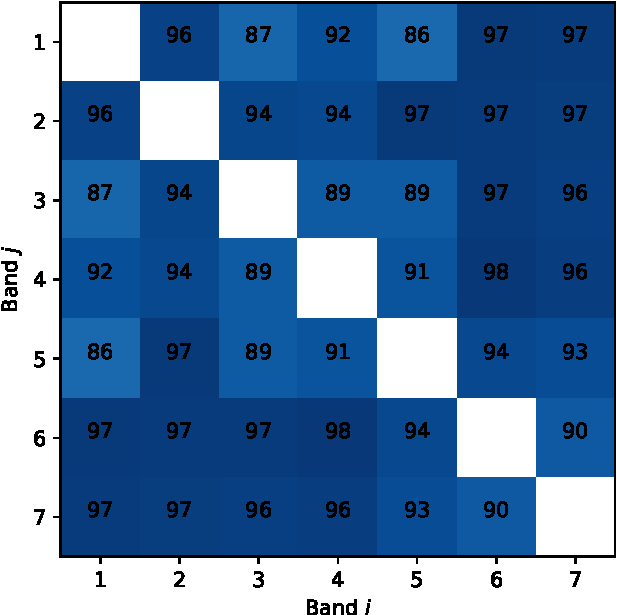
\includegraphics[width=0.9\linewidth]{sup-crop.pdf} 
    \caption{Logarithm applied} 
    \label{fig7:a} 
    %\vspace{4ex}
  \end{subfigure}%% 
  \begin{subfigure}[b]{0.49\linewidth}
    \centering
    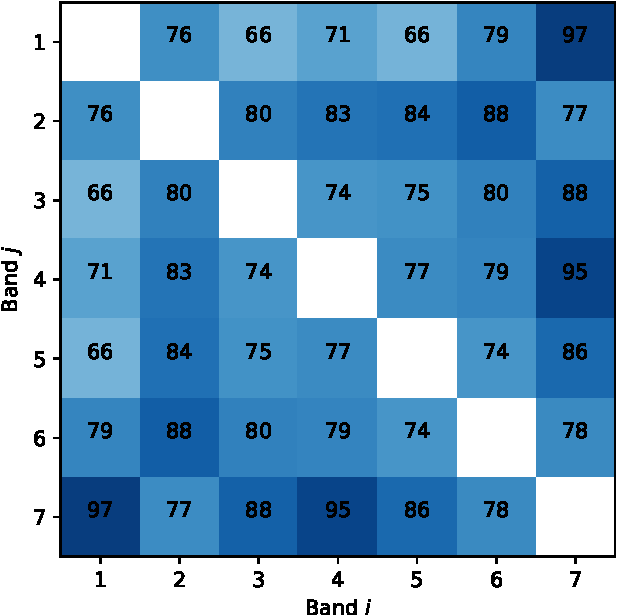
\includegraphics[width=0.9\textwidth]{un-crop.pdf} 
    \caption{Binary segmented image} 
    \label{fig7:b} 
    %\vspace{13ex}
    \end{subfigure} 
  \begin{subfigure}[b]{0.49\linewidth}
    \centering
    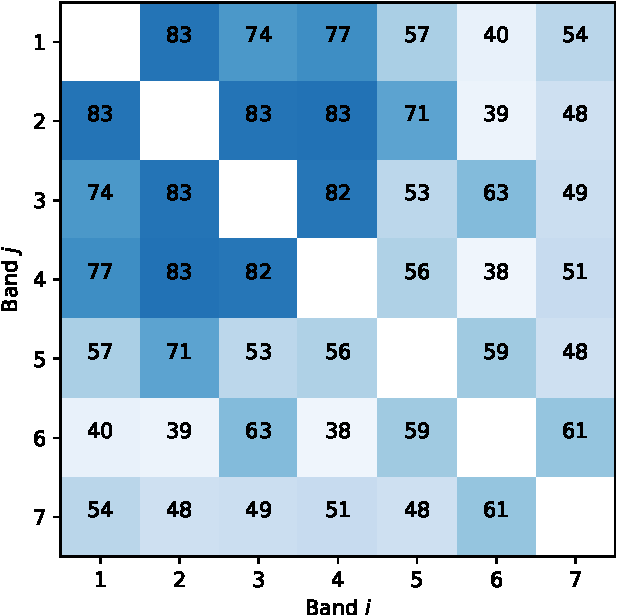
\includegraphics[width=0.9\textwidth]{kmeans-crop.pdf} 
    \caption{Hough Transform} 
    \label{fig7:c} 
  \end{subfigure}%%
  \begin{subfigure}[b]{0.49\linewidth}
    \centering
    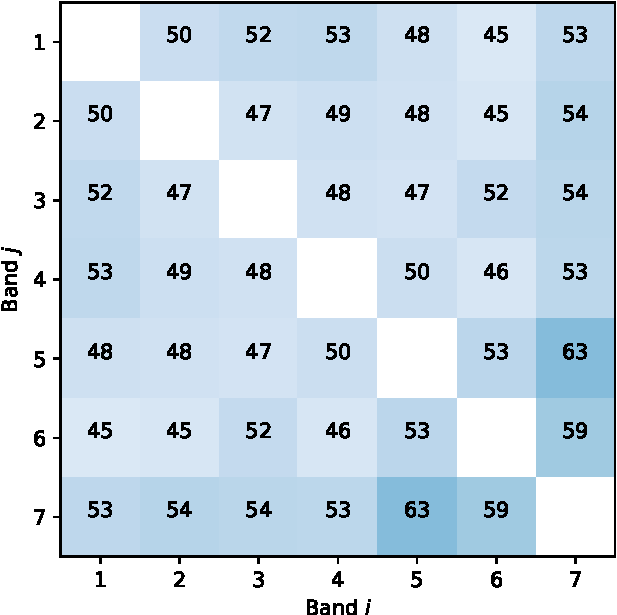
\includegraphics[width=0.9\textwidth]{gmm-crop.pdf} 
    \caption{Segmented image} 
    \label{fig7:d} 
  \end{subfigure} 
  \caption{c}
  \label{fig7} 
\end{figure*}





\section{Conclusion}
\label{sec:ref}
We presented a label agnostic feature extraction comparison framework in this paper. We demonstrated its usefulness by employing it and a case study to compare two feature extraction methods,
namely FFT and PCA (we also found that the PCA approach outperformed the FFT approach).

%List and number all bibliographical references at the end of the paper.  The references can be numbered in alphabetic order or in order of appearance in the document.  When referring to them in the text, type the corresponding reference number in square brackets as shown at the end of this sentence \cite{C2}.

% References should be produced using the bibtex program from suitable
% BiBTeX files (here: strings, refs, manuals). The IEEEbib.bst bibliography
% style file from IEEE produces unsorted bibliography list.
% -------------------------------------------------------------------------
\bibliographystyle{IEEEbib}
\bibliography{strings,refs}

\end{document}
